\chapter{Evaluation}~\label{cha:evaluation}
Once the application was deployed it had to be determined if the application met the requirements set out in the design phase. To do this the tests set out in Section~\ref{sec:test-design} were carried out.

\section{Primary Features}
These tests relate to the two primary feature tests set out in Section~\ref{sec:test-design}. These were the most crucial without which it would be hard to consider the application a success.

\subsection{Album Scanning}
The album scanning mechanism consisted of two separate APIs and so the evaluation here focuses on if the method used, that is directly searching for the album using the best guess or website titles, was successful. In total fifteen albums were used (all of which can be found in Appendix~\ref{apd:test_albums}), with six images used for each album: four rotations, one blurred, and one scaled down. There was a preference for self taken images given these would not be pre-indexed by search engines as would be more representative of the images a user would take.
Results were deemed correct for the reverse image search if they contained the exact album name and results for the Spotify search were deemed correct if the exact correct album was returned.

\subsubsection{Results}
The results are split into two sets. The first, seen in Figure~\ref{fig:album-scanning-results-ris}, shows the accuracy of the Google Reverse Image search API. Though this is treated as a black box that cannot be changed it is useful to see how accurate it is. The second set, seen in Figure~\ref{fig:album-scanning-results-spotify}, shows the accuracy of the Spotify search API only counting the times the results from the reverse image search were correct to evaluate it in isolation.

\begin{figure} [H]
    \centering
    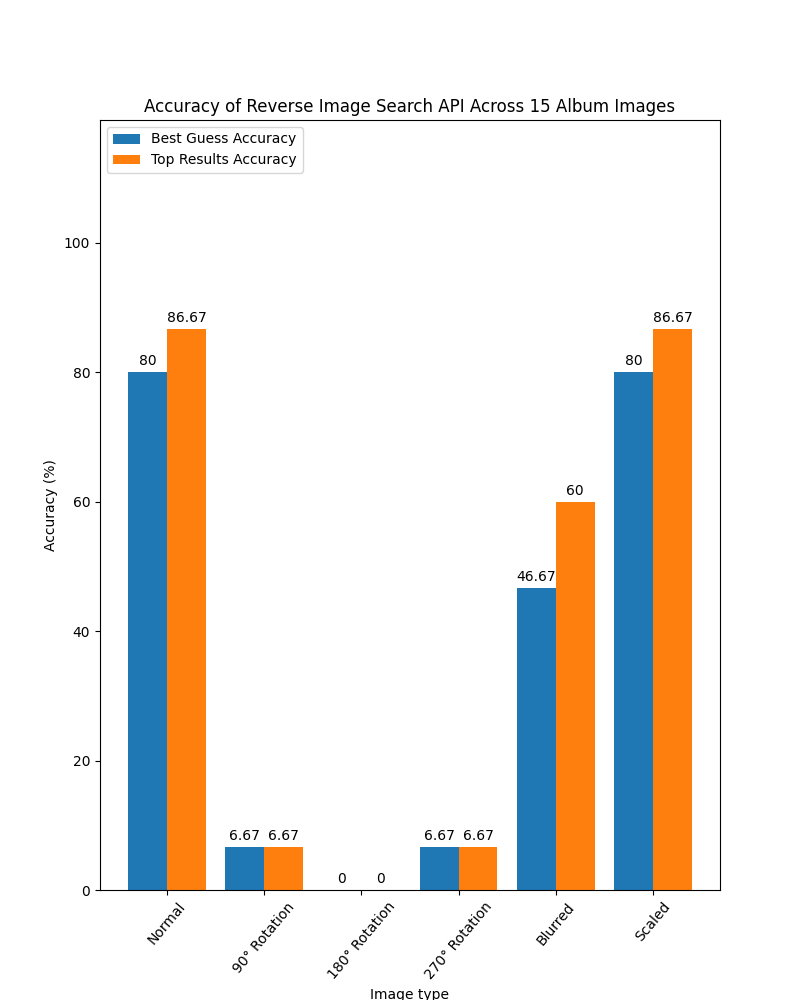
\includegraphics[width=0.8\textwidth]{figures/evaluation_graphs_ris.png}
    \caption{Accuracy of Reverse Image Search}
    \label{fig:album-scanning-results-ris}
\end{figure}

The results from the reverse image search were not as good as hoped. Compared to a hoped $95\%$ accuracy, for normal images, only a $80\%$ accuracy was measured for using the best guess and a $86.67\%$ accuracy for using website titles. The results for the rotations of the images were particularly poor. The only albums to be correctly identified were albums with artwork that was itself rotated.

The results do show that the scatter-shot approach using website titles was equally or more successful in all categories, so its presence in the application is beneficial.

\begin{figure} [H]
    \centering
    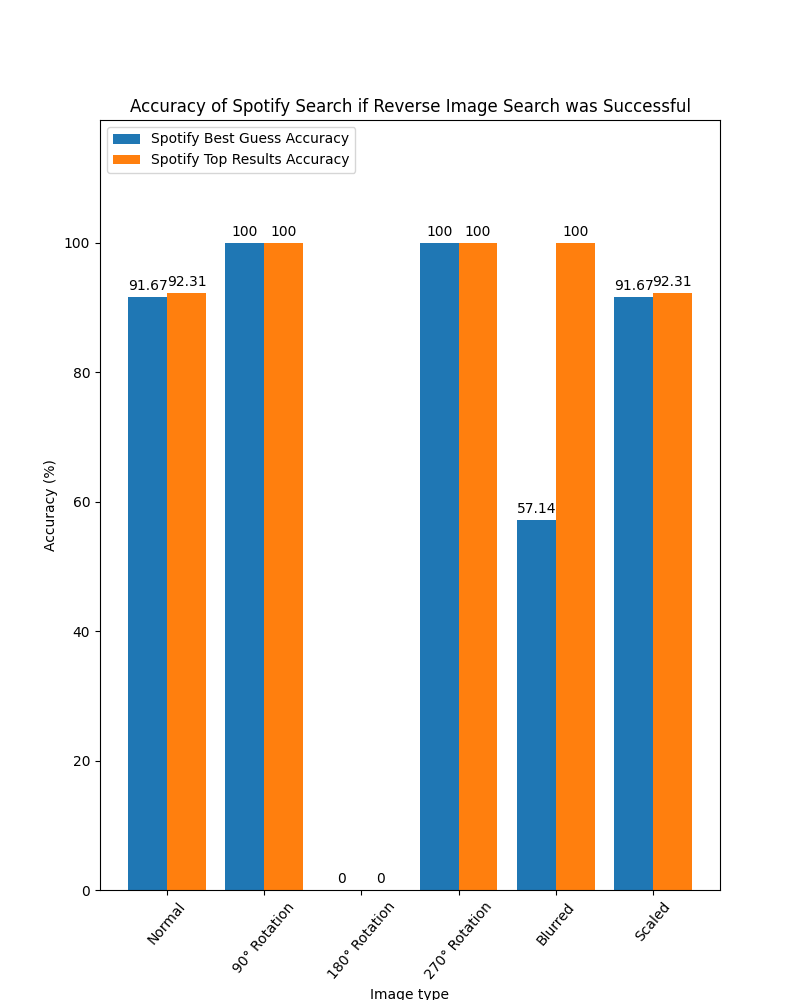
\includegraphics[width=0.8\textwidth]{figures/evaluation_graphs_spotify.png}
    \caption{Accuracy of Spotify Search}
    \label{fig:album-scanning-results-spotify}
\end{figure}

The results from the Spotify search were much better. If provided with a correct image search result, the Spotify search was able to find the correct album $91.67\%$ of the time for best guess searches and $92.31\%$ of the time for website titles.

This implies the chosen method of directly taking outputs from the reverse image search API and using them as inputs for the Spotify search API was broadly successful even though it did not reach the hoped $95\%$ accuracy.

The overall takeaway from this is the limiting factor of the accuracy of the system is the reverse image search and so by extension any improvements to the system should focus on improving this. However, since the Google API is a black box the only improvements that could be made would be to provide a better input.

This could potentially be done by pre-processing the image and attempting to remove the background via segmentation [TODO: Add reference to segmentation] or if it cannot be done automatically getting the user to crop down the image to just the album cover. Though these improvements would require potential user interface changes and increase the time taken to scan an album.


\subsection{Album Playback}

\section{User Interface}

\section{Development Practices}

%TODO: Talk about how the testing might not be 100% accurate


%Cite some references \cite{dyke1994, latex2012}
